\subsubsection{Séquentiel}
L'opérateur séquentiel, aussi abrégé {\em S} dans Taggre, est un opérateur très simple à comprendre.
%
Son but est de de fusionner les tâches qui n'apportent pas de parallélisme.
%
En agrégeant ces tâches ensemble, on ne perd pas de parallélisme et on économise le temps d'ordonnancement des tâches.
%
On peut reconnaître un groupe de deux tâches séquentielles par le fait qu'une des tâches n'as qu'un seul successeur et l'autre tâche n'as qu'un seul prédécesseur (Fig~\ref{fig:algo_S}).
%
%   (-_-)   %
\begin{figure}[t!]
  \centering
  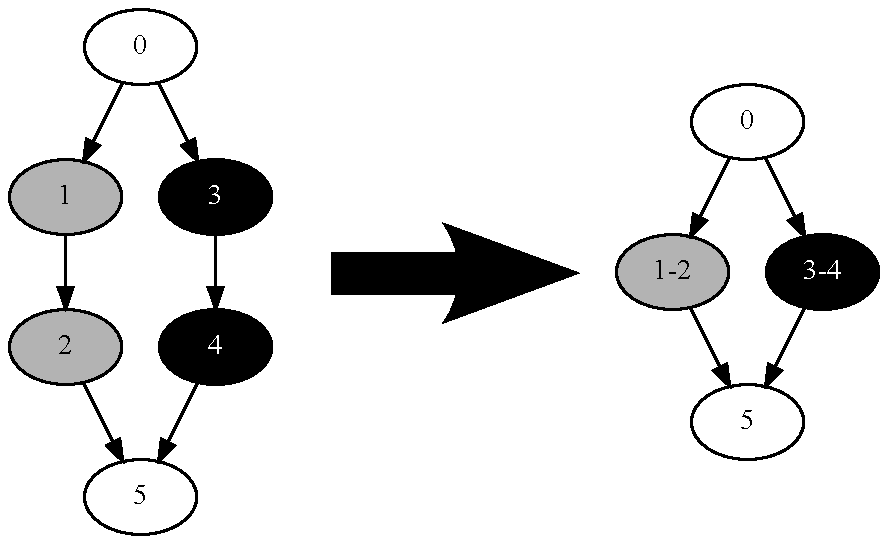
\includegraphics[width=0.7\textwidth]{algo_S}
  \caption{Exemple d'agrégation par l'opérateur séquentiel.}
  \label{fig:algo_S}
\end{figure}
